% Options for packages loaded elsewhere
\PassOptionsToPackage{unicode}{hyperref}
\PassOptionsToPackage{hyphens}{url}
%
\documentclass[
  12pt,
]{article}
\usepackage{amsmath,amssymb}
\usepackage{lmodern}
\usepackage{setspace}
\usepackage{iftex}
\ifPDFTeX
  \usepackage[T1]{fontenc}
  \usepackage[utf8]{inputenc}
  \usepackage{textcomp} % provide euro and other symbols
\else % if luatex or xetex
  \usepackage{unicode-math}
  \defaultfontfeatures{Scale=MatchLowercase}
  \defaultfontfeatures[\rmfamily]{Ligatures=TeX,Scale=1}
\fi
% Use upquote if available, for straight quotes in verbatim environments
\IfFileExists{upquote.sty}{\usepackage{upquote}}{}
\IfFileExists{microtype.sty}{% use microtype if available
  \usepackage[]{microtype}
  \UseMicrotypeSet[protrusion]{basicmath} % disable protrusion for tt fonts
}{}
\makeatletter
\@ifundefined{KOMAClassName}{% if non-KOMA class
  \IfFileExists{parskip.sty}{%
    \usepackage{parskip}
  }{% else
    \setlength{\parindent}{0pt}
    \setlength{\parskip}{6pt plus 2pt minus 1pt}}
}{% if KOMA class
  \KOMAoptions{parskip=half}}
\makeatother
\usepackage{xcolor}
\usepackage[margin=1in]{geometry}
\usepackage{longtable,booktabs,array}
\usepackage{calc} % for calculating minipage widths
% Correct order of tables after \paragraph or \subparagraph
\usepackage{etoolbox}
\makeatletter
\patchcmd\longtable{\par}{\if@noskipsec\mbox{}\fi\par}{}{}
\makeatother
% Allow footnotes in longtable head/foot
\IfFileExists{footnotehyper.sty}{\usepackage{footnotehyper}}{\usepackage{footnote}}
\makesavenoteenv{longtable}
\usepackage{graphicx}
\makeatletter
\def\maxwidth{\ifdim\Gin@nat@width>\linewidth\linewidth\else\Gin@nat@width\fi}
\def\maxheight{\ifdim\Gin@nat@height>\textheight\textheight\else\Gin@nat@height\fi}
\makeatother
% Scale images if necessary, so that they will not overflow the page
% margins by default, and it is still possible to overwrite the defaults
% using explicit options in \includegraphics[width, height, ...]{}
\setkeys{Gin}{width=\maxwidth,height=\maxheight,keepaspectratio}
% Set default figure placement to htbp
\makeatletter
\def\fps@figure{htbp}
\makeatother
\setlength{\emergencystretch}{3em} % prevent overfull lines
\providecommand{\tightlist}{%
  \setlength{\itemsep}{0pt}\setlength{\parskip}{0pt}}
\setcounter{secnumdepth}{-\maxdimen} % remove section numbering
\newlength{\cslhangindent}
\setlength{\cslhangindent}{1.5em}
\newlength{\csllabelwidth}
\setlength{\csllabelwidth}{3em}
\newlength{\cslentryspacingunit} % times entry-spacing
\setlength{\cslentryspacingunit}{\parskip}
\newenvironment{CSLReferences}[2] % #1 hanging-ident, #2 entry spacing
 {% don't indent paragraphs
  \setlength{\parindent}{0pt}
  % turn on hanging indent if param 1 is 1
  \ifodd #1
  \let\oldpar\par
  \def\par{\hangindent=\cslhangindent\oldpar}
  \fi
  % set entry spacing
  \setlength{\parskip}{#2\cslentryspacingunit}
 }%
 {}
\usepackage{calc}
\newcommand{\CSLBlock}[1]{#1\hfill\break}
\newcommand{\CSLLeftMargin}[1]{\parbox[t]{\csllabelwidth}{#1}}
\newcommand{\CSLRightInline}[1]{\parbox[t]{\linewidth - \csllabelwidth}{#1}\break}
\newcommand{\CSLIndent}[1]{\hspace{\cslhangindent}#1}
% \documentclass[11pt]{article}
\usepackage[sc]{mathpazo} %Like Palatino with extensive math support
\usepackage{fullpage}
\usepackage[authoryear,sectionbib,sort]{natbib}
\linespread{1.7}
\usepackage[utf8]{inputenc}
\usepackage{lineno}
\usepackage{titlesec}
\titleformat{\section}[block]{\Large\bfseries\filcenter}{\thesection}{1em}{}
\titleformat{\subsection}[block]{\Large\itshape\filcenter}{\thesubsection}{1em}{}
\titleformat{\subsubsection}[block]{\large\itshape}{\thesubsubsection}{1em}{}
\titleformat{\paragraph}[runin]{\itshape}{\theparagraph}{1em}{}[. ]
\usepackage{fancyhdr}
\pagestyle{fancy}
\usepackage{multirow} % for merging rows in tables
\usepackage{caption} % for \captionsetup{labelformat=empty}
\usepackage{nopageno}

%%%%%%%%%%%%%%%%%%%%%
% Header
%%%%%%%%%%%%%%%%%%%%%
%
% Customize the line below with the last name of your first author and
% the short title of your MS. You can comment authorship information out
% while your MS is undergoing double-blind review.
%
\rhead{Supplement to Muir et al., ``Constraints on stomatal anatomy,'' \textit{Am.~Nat.}}
\setlength{\headsep}{0.3in}  
\lhead{} 

%%%%%%%%%%%%%%%%%%%%%
% Line numbering
%%%%%%%%%%%%%%%%%%%%%
%
% Please use line numbering with your initial submission and
% subsequent revisions. After acceptance, please turn line numbering
% off by adding percent signs to the lines %\usepackage{lineno} and
% to %\linenumbers{} and %\modulolinenumbers[3] below.
%
% To avoid line numbering being thrown off around math environments,
% the math environments have to be wrapped using
% \begin{linenomath*} and \end{linenomath*}
%
% (Thanks to Vlastimil Krivan for pointing this out to us!)

\title{Online Supplement: \\ 
How important are functional and developmental constraints on phenotypic evolution? An empirical test with the stomatal anatomy of flowering plants, \\ 
\textit{The~American~Naturalist} }

% This version of the LaTeX supplementary template was last updated on
% November 8, 2019.

%%%%%%%%%%%%%%%%%%%%%
% Authorship
%%%%%%%%%%%%%%%%%%%%%
% Please remove authorship information while your paper is under review,
% unless you wish to waive your anonymity under double-blind review. You
% will need to add this information back in to your final files after
% acceptance.
%
% Once accepted for publication, author-supplied PDFs should have a 
% title page that includes (at least) the authors' names, the title of 
% the MS, and the name of the journal. It should also have a header and
% page numbers.

\author{Christopher D. Muir$^{1,\ast}$ \\ 
Miquel \`{A}ngel Conesa$^{2}$ \\ 
Jeroni Galm\'{e}s$^{2}$ \\
Varsha S. Pathare$^{3}$ \\
Patricia Rivera$^{4}$ \\
Rosana López Rodríguez$^{5}$ \\
Teresa Terrazas$^{4}$ \\
Dongliang Xiong$^{6}$ 
}

\date{}
\ifLuaTeX
  \usepackage{selnolig}  % disable illegal ligatures
\fi
\IfFileExists{bookmark.sty}{\usepackage{bookmark}}{\usepackage{hyperref}}
\IfFileExists{xurl.sty}{\usepackage{xurl}}{} % add URL line breaks if available
\urlstyle{same} % disable monospaced font for URLs
\hypersetup{
  hidelinks,
  pdfcreator={LaTeX via pandoc}}

\begin{document}



\setstretch{1}
\maketitle

\noindent{} 1. School of Life Sciences, University of Hawaii at Mānoa, Honolulu, HI 96822, USA;

\noindent{} 2. Research Group on Plant Biology under Mediterranean Conditions, Departament de Biologia, Universitat de les Illes Balears, Ctra. Valldemossa km 7.5, E-07122, Palma, Spain;

\noindent{} 3. School of Biological Sciences, Washington State University, Pullman, WA 99164-4236, USA;

\noindent{} 4. Departamento de Botánica, Instituto de Biología, Universidad Nacional Autónoma de México, Apartado Postal 70‑367, 04510 Mexico City, Mexico;

\noindent{} 5. Departamento de Sistemas y Recursos Naturales, Universidad Politécnica de Madrid, 28040 Madrid, Spain;

\noindent{} 6. National Key Laboratory of Crop Genetic Improvement, MOA Key Laboratory of Crop Ecophysiology and Farming System in the Middle Reaches of the Yangtze River, College of Plant Science and Technology, Huazhong Agricultural University, Wuhan, Hubei 430070, China.

\noindent{} \(\ast\) Corresponding author; e-mail: \href{mailto:cdmuir@hawaii.edu}{\nolinkurl{cdmuir@hawaii.edu}}

\begin{table}
  \captionsetup{labelformat=empty}
  \caption{}
  \label{tab:traits}
\end{table}

\begin{figure}[ht]
  \captionsetup{labelformat=empty}
  \caption{}
  \label{fig:concepts}
\end{figure}

\begin{figure}[ht]
  \captionsetup{labelformat=empty}
  \caption{}
  \label{fig:h3}
\end{figure}

\begin{figure}[ht]
  \captionsetup{labelformat=empty}
  \caption{}
  \label{fig:h1_raw}
\end{figure}

\begin{figure}[ht]
  \captionsetup{labelformat=empty}
  \caption{}
  \label{fig:h1}
\end{figure}

\begin{figure}[ht]
  \captionsetup{labelformat=empty}
  \caption{}
  \label{fig:h2_raw}
\end{figure}

\begin{figure}[ht]
  \captionsetup{labelformat=empty}
  \caption{}
  \label{fig:h2}
\end{figure}

\renewcommand\thefigure{S\arabic{figure}}    
\renewcommand\thetable{S\arabic{table}}    
\renewcommand\theequation{S\arabic{equation}}    
\setcounter{figure}{0}    
\setcounter{table}{0}    
\setcounter{equation}{0}

\begin{figure}[ht]
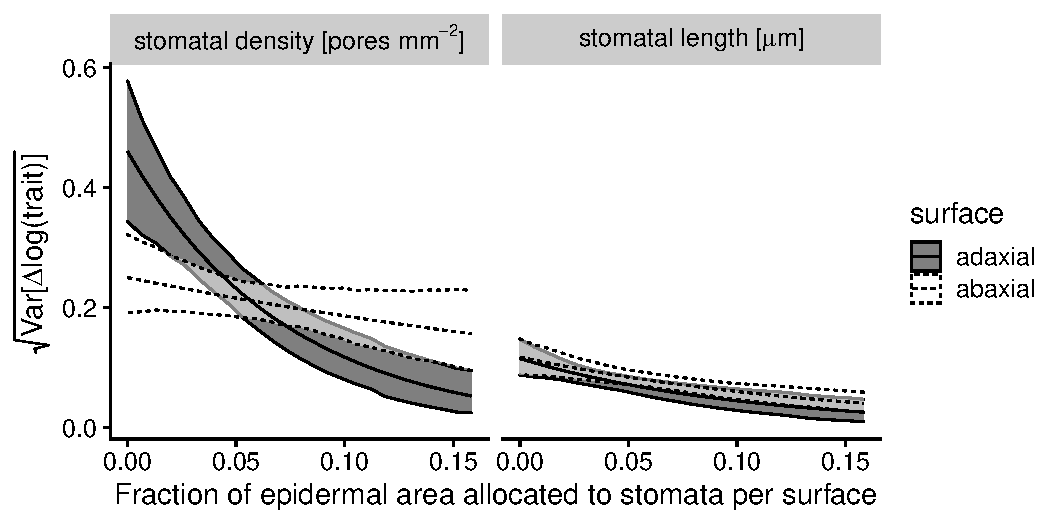
\includegraphics[width=\textwidth]{../figures/fs-sigma.pdf}
\caption{The variance in evolutionary divergence ($y$-axis, $\textrm{Var}[\Delta \textrm{log(trait)}]$) declines the fraction of epidermal space allocated to stomata per surface ($x$-axis, $f_S$) increases. Within each ribbon, the middle line is the median estimate and the outer lines are the 95\% HPD intervals. The slope is significantly less than 0 for adaxial stomatal density and stomatal length of both surface (Table \ref{tab:h3output}). Results for the standard deviation, which is the square-root of the variance, are shown.}
\label{fig:fs-sigma}
\end{figure}

\begin{figure}[ht]
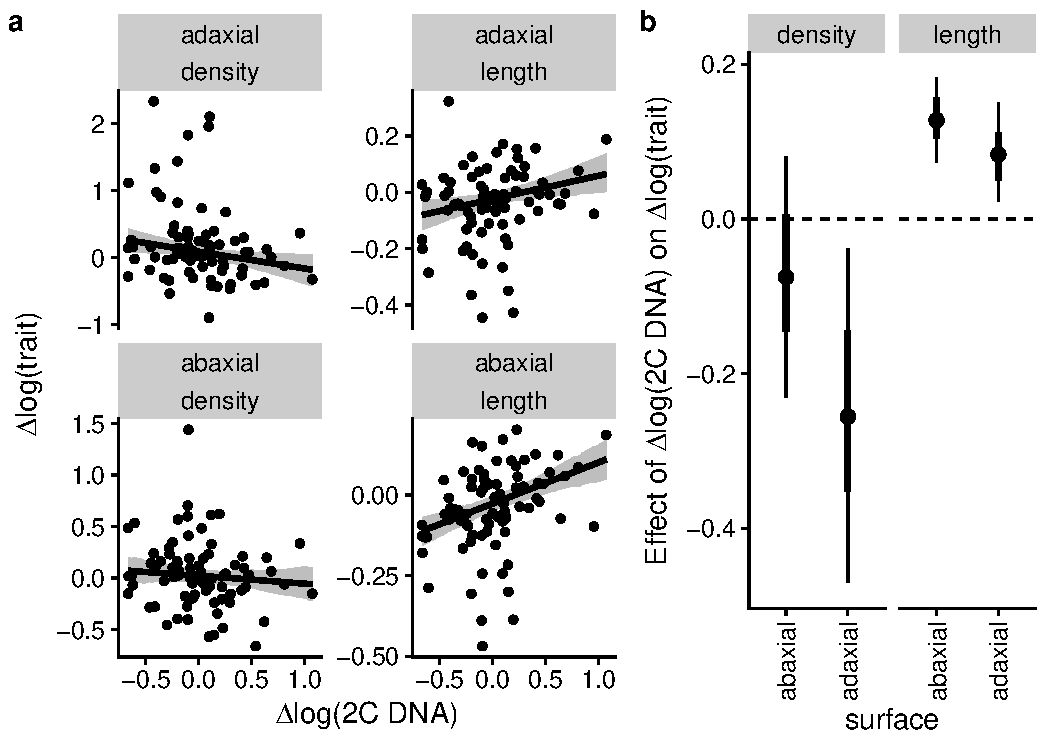
\includegraphics[width=\textwidth]{../figures/genome.pdf}
\caption{Evolutionary divergence in genome size (2C DNA content) is associated with guard cell length, but less so stomatal density. (a) Data from 79 phylogenetically independent contrasts of change in log(2C DNA) ($x$-axis) and change in log(trait) ($y$-axis) for abaxial (lower panels) and adaxial (upper panels) leaf surfaces. Each contrast is shown by black points and every contrast appears on all panels. Black lines are the median predicted trait divergence and grey ribbons are the model-estimated 95\% HPD confidence bands. (b) Parameter estimates (points), 66\% (thick lines), and 95\% HPD intervals for estimates of the effect of change in log(2C DNA) on change in log(trait). HPD intervals that do not overlap zero indicate that divergence in genome size is associated with divergence in stomatal anatomy. Reported parameter estimates are conditioned on zero time since divergence between taxa (see \protect\hyperlink{results}{Results}).}
  \label{fig:genome}
\end{figure}

\clearpage

\begin{center}
  Table S1 is a csv file uploaded with this manuscript and will be included as an online supplement upon publication.
\end{center}

\begin{table}
\caption{\label{tab:pair_div}Final data set of 236 taxon pairs for analysis. $\tt{tree\_node}$ is the node of the common ancestor of the taxon pair $\tt{sp1}$ and $\tt{sp2}$ in the phylogeny (Notes S3). $\tt{pair\_age}$ is the time in millions of years since taxa split. The remaining columns are the trait divergence (log-scale) between taxa ($\Delta \text{log(trait)}$).}
\end{table}

\begin{table}[ht]
\caption{\label{tab:h3output} Parameter estimates and 95\% highest posterior density (HPD) intervals for the effect of  $f_S$ on trait divergence. For each trait ($D_\mathrm{ab}$, $D_\mathrm{ad}$, $L_\mathrm{ab}$, $L_\mathrm{ad}$) we estimated the coefficient of $f_S$ on the standard deviation of $\Delta \text{log(trait)}$ on a log-link scale. Other model parameter estimates and confidence intervals can be found in the saved model output located in the archived online repository (see \protect\hyperlink{results}{Data avaibility}).}
\begin{center}
\begin{tabular}{lll}

  \toprule
  Trait(s) & Estimate & 95\% HPD interval \\
  \midrule
  
  \multicolumn{3}{l}{Effect of $f_S$ on standard deviation of $\Delta \text{log(trait)}$} \\
  \multicolumn{3}{l}{log-link scale} \\
  \\
  $D_\mathrm{ab}$ &  -3.2  & $[-6.6,0.75]$  \\
  $D_\mathrm{ad}$ & -12.0  & $[-17,-6.9]$  \\
  $L_\mathrm{ab}$ &  -6.7  & $[-10,-2.9]$  \\
  $L_\mathrm{ad}$ &  -9.8  & $[-16,-4.1]$  \\
  \\

\bottomrule

\end{tabular}
\end{center}
\end{table}

\begin{table}[ht]
\caption{\label{tab:h12output} Parameter estimates and 95\% highest posterior density (HPD) intervals for the (co)variance of trait divergence. For each trait ($D_\mathrm{ab}$, $D_\mathrm{ad}$, $L_\mathrm{ab}$, $L_\mathrm{ad}$) we estimated the average (median) divergence between taxon pairs, denoted $\Delta \text{log(trait)}$. See Table \ref{tab:traits} for symbol definitions. The second section is the standard deviation of $\Delta \text{log(trait)}$. The third section is the estimated coefficient of pair age (millions of years) on the standard deviation on a log-link scale. The fourth section is the estimated correlation coefficient between $\Delta \text{log(trait)}$ of all pairwise trait combinations. The final section is the estimated $\nu$ family of the Student $t$ distribution.}
\begin{center}
\begin{tabular}{lll}

  \toprule
  Trait(s) & Estimate & 95\% HPD interval \\
  \midrule
  
  \multicolumn{3}{l}{Average $\Delta \text{log(trait)}$} \\
  \\
  $D_\mathrm{ab}$ &  0.00180  & $[-0.029,0.035]$  \\
  $D_\mathrm{ad}$ &  0.00069  & $[-0.045,0.047]$  \\
  $L_\mathrm{ab}$ & -0.00620  & $[-0.019,0.0079]$  \\
  $L_\mathrm{ad}$ & -0.00760  & $[-0.021,0.0055]$  \\
  \\
  \multicolumn{3}{l}{Standard deviation of $\Delta \text{log(trait)}$} \\
  \\
  $D_\mathrm{ab}$ & 0.220  & $[0.19,0.26]$  \\
  $D_\mathrm{ad}$ & 0.300  & $[0.25,0.35]$  \\
  $L_\mathrm{ab}$ & 0.087  & $[0.075,0.1]$  \\
  $L_\mathrm{ad}$ & 0.084  & $[0.073,0.098]$  \\
  \\
  \multicolumn{3}{l}{Effect of pair age on standard deviation of $\Delta \text{log(trait)}$} \\
  \multicolumn{3}{l}{log-link scale} \\
  \\
  $D_\mathrm{ab}$ & 0.004  & $[-0.0034,0.013]$  \\
  $D_\mathrm{ad}$ & 0.013  & $[0.0047,0.022]$  \\
  $L_\mathrm{ab}$ & 0.012  & $[0.0057,0.02]$  \\
  $L_\mathrm{ad}$ & 0.013  & $[0.0064,0.019]$  \\
  \\
  \multicolumn{3}{l}{Correlation between $\Delta \text{log(trait)}$} \\
  \\
  $D_\mathrm{ab}-D_\mathrm{ad}$ & 
   0.34  & $[0.21,0.45]$  \\
  $D_\mathrm{ab}-L_\mathrm{ab}$ & 
  -0.56  & $[-0.65,-0.45]$  \\
  $D_\mathrm{ab}-L_\mathrm{ad}$ & 
  -0.46  & $[-0.57,-0.35]$  \\
  $D_\mathrm{ad}-L_\mathrm{ab}$ & 
  -0.37  & $[-0.48,-0.25]$  \\
  $D_\mathrm{ad}-L_\mathrm{ad}$ & 
  -0.41  & $[-0.52,-0.31]$  \\
  $L_\mathrm{ab}-L_\mathrm{ad}$ & 
   0.87  & $[0.83,0.91]$  \\
  \\
  \multicolumn{3}{l}{Student $t$ family parameter $\nu$} \\
  \\
  $-$ & 3.4  & $[2.5,4.4]$  \\

\bottomrule

\end{tabular}
\end{center}
\end{table}

\clearpage

\hypertarget{notes-s1-theory-connecting-developmental-function-constraint-and-integration}{%
\subsection{Notes S1: Theory connecting developmental function, constraint, and integration}\label{notes-s1-theory-connecting-developmental-function-constraint-and-integration}}

Below we provide a conceptual background to motivate the derivation of a stomatal developmental function. We then derive predictions for how stomatal size and density should diverge with or without developmental constraint. We then explain why comparing evolutionary divergence of lower and upper stomatal anatomy provides an important additional line of evidence on the contribution of developmental integration to phenotypic macroevolution. Fig. \ref{fig:developmental-integration} is a graphical summary of our analysis.

\begin{figure}[ht]
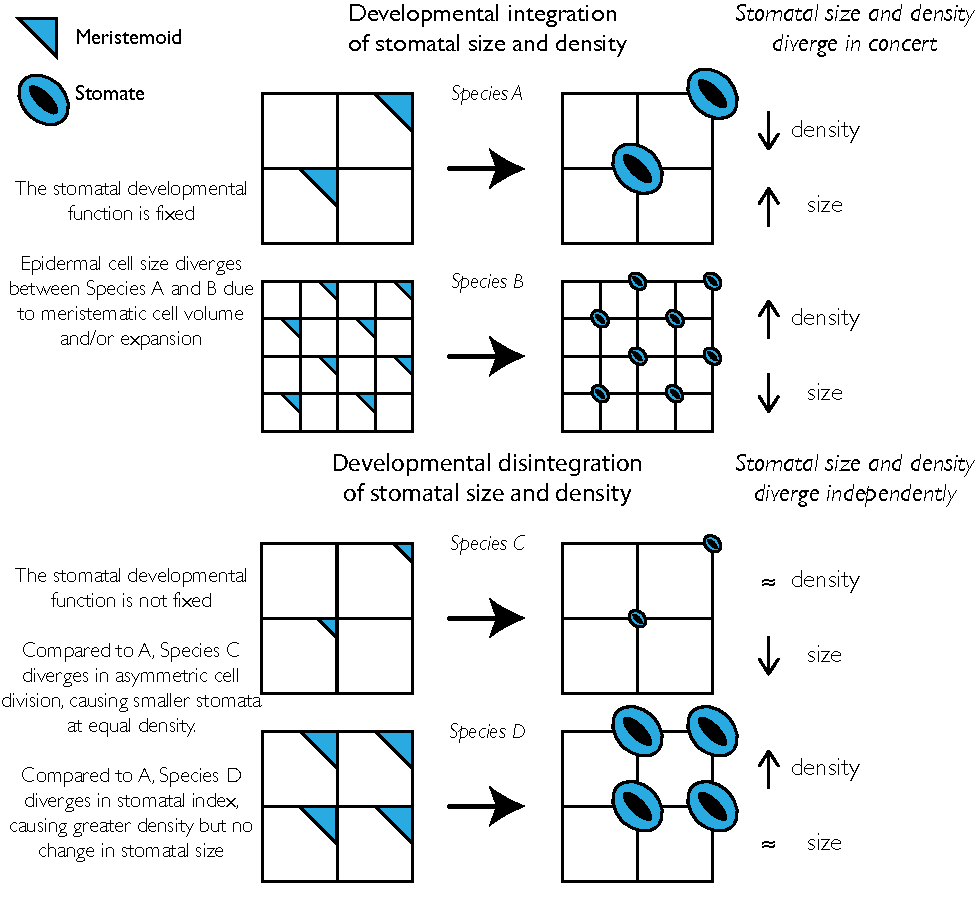
\includegraphics[width=\textwidth]{../figures/developmental-integration.pdf}
\caption{Graphical summary describing contrasting predictions of developal integration and disintegration hypotheses. Meristematic cell volume and expansion determine the epidermal (white squares) and guard meristemoid (blue triangles) cell sizes before final differentiation into stomata. Because the developmental function is fixed, larger meristematic cell volume and greater expansion result in larger stomata at lower density (Species A); smaller meristematic cell volume and less expansion result in smaller stomata at higher density (Species B). Stomatal size and density can evolve independently if the developmental function is not fixed. Species C diverges in size but not density by allocating less volume to the guard meristemoid during asymmetic cell division. Species D diverges in density but not size by increasing stomatal index.}
\label{fig:developmental-integration}
\end{figure}

\hypertarget{conceptual-background}{%
\subsubsection{Conceptual background}\label{conceptual-background}}

Developmental integration in stomatal anatomy is plausible because epidermal pavement cells and stomata share an early developmental history, originating from the same leaf meristem tissue. If all other factors are held constant, meristematic cell volume, which is largely determined by genome size (\protect\hyperlink{ref-simova_geometrical_2012}{Šímová and Herben 2012}), and early expansion rate increase both epidermal cell and stomatal area proportionally. This mechanically decreases stomatal density because the same number of stomata per epidermal cell (stomatal index) are spread farther apart by larger epidermal cells. Developmental integration between stomatal size and density arises naturally if meristematic cell volume and/or expansion rate evolve, but the remaining steps of stomatal development are fixed. As described in detail below, we mathematically formalize these later steps in stomatal development into a `developmental function' inspired by Wagner (\protect\hyperlink{ref-wagner_multivariate_1989}{1989}). Wagner's used a developmental function to map genetic variance onto phenotypic variance. The developmental function can cause a disposition for phenotypic covariance, depending on the amount of pleiotropy. For example, genetic changes in a growth factor could be highly pleiotropic, simultaneously altering the size of many tissues. Wagner used the developmental function to model microevolution, but if we suppose that the developmental function is fixed over long time periods, it can be used to predict macroevolutionary divergence under developmental constraint. If the developmental function is fixed or highly constrained, species may never possess the genetic variation to access regions of phenotypic space. If the developmental function itself can evolve readily, then traits should be able to evolve independently given sufficient time for mutation, selection, and divergence. Finding that the developmental function is malleable would lend less credence to the importance of developmental constraint and lend more credence to selective hypotheses.

The stomatal developmental function is probably not fixed, potentially allowing for independent evolution of stomatal size and density. The conceptual model of stomatal development by Dow and Bergmann (\protect\hyperlink{ref-dow_patterning_2014}{2014}) identifies three key cell division types that could shape stomatal density and size. First, asymmetric division of undifferentiated epidermal cells forms the guard cell meristemoid. Larger allocation to and/or greater expansion of the meristemoid as it matures to a guard mother cell increases stomatal size without affecting density. Second, spacing divisions in developing epidermal cells increase stomatal density and index while maintaining spacing. Third, amplifying divisions generate more epidermal cells without further differentiation of stomata, decreasing stomatal density and index. Changing the probability of spacing and amplifying divisions affects stomatal density without changing size.

Below we formalize these models of developmental (dis)integration to address the following two questions:

\begin{enumerate}
\def\labelenumi{\arabic{enumi}.}
\item
  How would stomatal size and density (co)diverge if the developmental function is fixed? We refer to this as the `developmental integration' hypothesis.
\item
  How would stomatal size and density (co)diverge if the developmental function is not fixed? We refer to this as the `developmental disintegration' hypothesis.
\end{enumerate}

\hypertarget{theory}{%
\subsubsection{Theory}\label{theory}}

\hypertarget{a-developmental-function-for-stomatal-size-and-density}{%
\paragraph{A developmental function for stomatal size and density}\label{a-developmental-function-for-stomatal-size-and-density}}

In this section we derive a stomatal developmental function by extending the model of Sack and Buckley (\protect\hyperlink{ref-sack_developmental_2016}{2016}) in two ways. First, we provide an explicit, albeit simple, map from meristematic cell volume to stomatal size and density. Second, we use random variable algebra (\protect\hyperlink{ref-lynch_genetics_1998}{Lynch and Walsh 1998}) to derive expectations for the variance in stomatal anatomy among species. Sack and Buckley (\protect\hyperlink{ref-sack_developmental_2016}{2016}) consider three anatomical properties of a leaf surface, the projected epidermal cell area \(E\), the area of the stomatal apparatus \(S\), and the stomatal index \(I\):

\[I = \frac{n_S}{n_S + n_E}\]
\(n_S\) and \(n_E\) are the number of stomatal and other epidermal cells, respectively, on the leaf surface. Throughout this we supplement we focus on stomatal size (\(S\)) rather than guard cell length (\(L\)) because it is mathematically simpler. For comparison with our data on \(L\), we derive predictions using the fact that \(S = j L^2\) where \(j=0.5\) for non-grasses and 0.125 for grasses (\protect\hyperlink{ref-sack_developmental_2016}{Sack and Buckley 2016}).

Next, we assume that the area of epidermal cells and stomata are proportional to the meristematic cell volume \(M\):

\begin{align}
  E = & A M \\
  S = & B E = A B M
  \label{eq:eq1}
\end{align}

The coefficient \(A\) is determined by the early cell expansion and division rates, which we do not model explicitly. \(B\) is determined by the placement of the asymmetric cell division generating the guard mother cell (\protect\hyperlink{ref-bergmann_stomatal_2007}{Bergmann and Sack 2007}) and subsequent expansion of the guard cell meristemoid. For example, in \emph{Arabidopsis thaliana}, the cell volume of shoot meristematic cells is approximately 200 \(\mu\textrm{m}^3\) (\protect\hyperlink{ref-price_correlations_1973}{Price, Sparrow, and Nauman 1973}) and the epidermal and stomatal sizes are roughly 1000 and 250 \(\mu\textrm{m}^2\) (\protect\hyperlink{ref-dow_integrated_2014}{Dow, Bergmann, and Berry 2014}). Therefore \(A = \frac{1000~\mu\textrm{m}^3}{200 ~\mu\textrm{m}^2} = 5 \frac{\mu\textrm{m}^3}{\mu\textrm{m}^2}\) and \(B = \frac{250~\mu\textrm{m}^3}{1000 ~\mu\textrm{m}^2} = 0.25\).

Following Sack and Buckley (\protect\hyperlink{ref-sack_developmental_2016}{2016}) the stomatal density as a function of \(E\), \(S\), and \(I\) is:

\[D = \frac{I}{IS + (1 - I) E}\]

For analytical tractability, we use he first-order Taylor series approximation around \(I = 0\) because \(I\) is typically much closer to 0 than 1:

\[D \approx \frac{I}{E}\]

Below we show that this approximation accurately models the correlation in divergence between stomatal size and density by comparing it to random simulations (Fig. \ref{fig:check-approximation}.

Substituting Eqn. \ref{eq:eq1} into the above expression we obtain

\[D \approx \frac{I}{A M}\]

Now we can can derive a developmental function to map from \(M\) to \(S\) and \(D\). We assume that \(M\) is determined by genome size (\protect\hyperlink{ref-simova_geometrical_2012}{Šímová and Herben 2012}) and, possibly, other genetic and environmental factors that we do not track explicitly in our model. As with our empirical analysis, we work with the log-transformed values of \(S\) and \(D\) to linearize the developmental function. For brevity, let the lowercase variables be the log-transformed values of their uppercase counterparts (e.g.~\(d = \textrm{log}(D)\)). With these assumptions, we obtain:

\begin{align}
  d = &~i - a - m \\
  s = &~a + b + m 
  \label{eq:dev-fun}
\end{align}

\hypertarget{hypotheses}{%
\subsubsection{Hypotheses}\label{hypotheses}}

To address the two overarching questions posed above, we will use the theory in the previous section to derive predictions for two hypotheses. The developmental integration hypothesis can be thought of as a null hypothesis for how stomatal size and density diverge when the developmental function is fixed. The second hypothesis relaxes this constraint.

\begin{enumerate}
\def\labelenumi{\arabic{enumi}.}
\item
  Developmental integration hypothesis: the stomatal developmental function is fixed; divergence in stomatal size and density is caused only by divergence in meristematic cell volume and early expansion rate.
\item
  Developmental disintegration hypothesis: the stomatal developmental function is not fixed; divergence in stomatal size and density is caused by the combined divergence in meristematic cell volume, early expansion, and later cell divisions, the asymmetric, spacing, amplifying divisions discussed in the Conceptual background.
\end{enumerate}

\hypertarget{developmental-integration-hypothesis}{%
\paragraph{Developmental integration hypothesis}\label{developmental-integration-hypothesis}}

Under this hypothesis, meristematic cell volume and expansion rate integrate stomatal size and density because the developmental function is constrained. We know that meristematic cell volume can evolve as a product of genome size, so a natural null hypothesis is that \(m\) varies but the developmental parameters \(a\), \(b\), and \(i\) in Eqn. \ref{eq:dev-fun} are constant or vary little relative to \(m\). Let the divergence between taxa \(i\) and \(j\) be:

\begin{align}
  \Delta d = & d_j - d_i = (i_j - a_j - m_j) - (i_i - a_i - m_i) \\
    = & \Delta i - \Delta a - \Delta m \\
  \Delta s = & s_j - s_i = (a_j + b_j + m_j) - (a_i + b_i + m_i) \\
    = & \Delta a + \Delta b + \Delta m 
\end{align}

When developmental parameters are fixed \(\Delta a = \Delta b = \Delta i = 0\). This leads to integration between \(s\) and \(d\) mediated by \(m\) because \(\Delta s = \Delta m\), \(\Delta d = -\Delta m\), and \(\textrm{Cov}[\Delta s, \Delta d] = -\textrm{Var}[\Delta m]\). Strong developmental integration would also persist if \(\Delta b = \Delta i = 0\) but \(\Delta a \ne 0\). In that case, \(\Delta s = \Delta a + \Delta m\), \(\Delta d = -(\Delta a + \Delta m)\), and \(\textrm{Cov}[\Delta s, \Delta d] = -\textrm{Var}[\Delta a + \Delta m]\). In either case, the correlation between between \(\Delta d\) and \(\Delta s\) is \(-1\) because \(-\textrm{Cov}[\Delta s, \Delta d] = \textrm{Var}[\Delta d] = \textrm{Var}[\Delta s]\):

\begin{equation}
  \textrm{Corr}[\Delta d, \Delta s] = \frac{\textrm{Cov}[\Delta s, \Delta d]}{\sqrt{\textrm{Var}[\Delta d]} \sqrt{\textrm{Var}[\Delta s]}} = -1
\end{equation}

In summary, developmental constraint on stomatal index and allocation to guard mother cells during asymmetric cell division leads to developmental integration between stomatal size and density. Developmental integration can be mediated by either meristematic cell volume and/or epidermal cell expansion since they are colinear.

\hypertarget{developmental-disintegration-hypothesis}{%
\paragraph{Developmental disintegration hypothesis}\label{developmental-disintegration-hypothesis}}

Here we show that developmental disintegration is mediated by divergence in stomatal index and asymmetric cell division. In conceptual models of stomatal development (\protect\hyperlink{ref-dow_patterning_2014}{Dow and Bergmann 2014}), asymmetric division forms the meristemoid to the guard mother cell. After asymmetric division, spacing divisions increase stomatal density and index whereas amplifying divisions decrease both quantities. Above we assumed these processes were constrained; here we relax that assumption. First, we assume that \(\Delta b = 0\) and \(\Delta i \ne 0\). Further, we assume for simplicity that there is no covariance in divergence between \(m\) and \(i\) (\(\textrm{Cov}[\Delta i, \Delta m] = 0\). Using random variable algebra, the (co)variance and correlation between divergence in stomatal density and size are:

\begin{align}
  \textrm{Var}[\Delta d] = & \textrm{Var}[\Delta i] + \textrm{Var}[\Delta m] \\
  \textrm{Var}[\Delta s] = & \textrm{Var}[\Delta m] \\
  \textrm{Cov}[\Delta d, \Delta s] = & -\textrm{Var}[\Delta m] \\
  \textrm{Corr}[\Delta d, \Delta s] = & -\frac{\textrm{Var}[\Delta m]}{\sqrt{\textrm{Var}[\Delta i] + \textrm{Var}[\Delta m]}\sqrt{\textrm{Var}[\Delta m]}} \label{eq:corr-ds1}
\end{align}

Compared to the developmental integration hypothesis, variation in stomatal index leads to greater variation in stomatal density and disintegration (lower correlation) between density and size. The approximation in Eqn. \ref{eq:corr-ds1} matches simulated values well for realistic values of stomatal index (Fig. \ref{fig:check-approximation}).

Next, we switch our assumptions such that \(\Delta b \ne 0\) and \(\Delta i = 0\). We again make the simplifying assumption that there is no covariance in divergence between \(m\) and \(b\) (\(\textrm{Cov}[\Delta b, \Delta m] = 0\). The (co)variance and correlation between stomatal density and size are:

\begin{align}
  \textrm{Var}[\Delta d] = & \textrm{Var}[\Delta b] + \textrm{Var}[\Delta m] \\
  \textrm{Var}[\Delta s] = & \textrm{Var}[\Delta m] \\
  \textrm{Cov}[\Delta d, \Delta s] = & -\textrm{Var}[\Delta m] \\
  \textrm{Corr}[\Delta d, \Delta s] = & -\frac{\textrm{Var}[\Delta m]}{\sqrt{\textrm{Var}[\Delta m]}\sqrt{\textrm{Var}[\Delta b] + \textrm{Var}[\Delta m]}}
\end{align}

As with stomatal index, variation in asymmetric cell division also causes developmental disintegration. The key difference is that disintegration is driven by greater variation in stomatal size rather than density.

\begin{figure}[ht]
\begin{center}
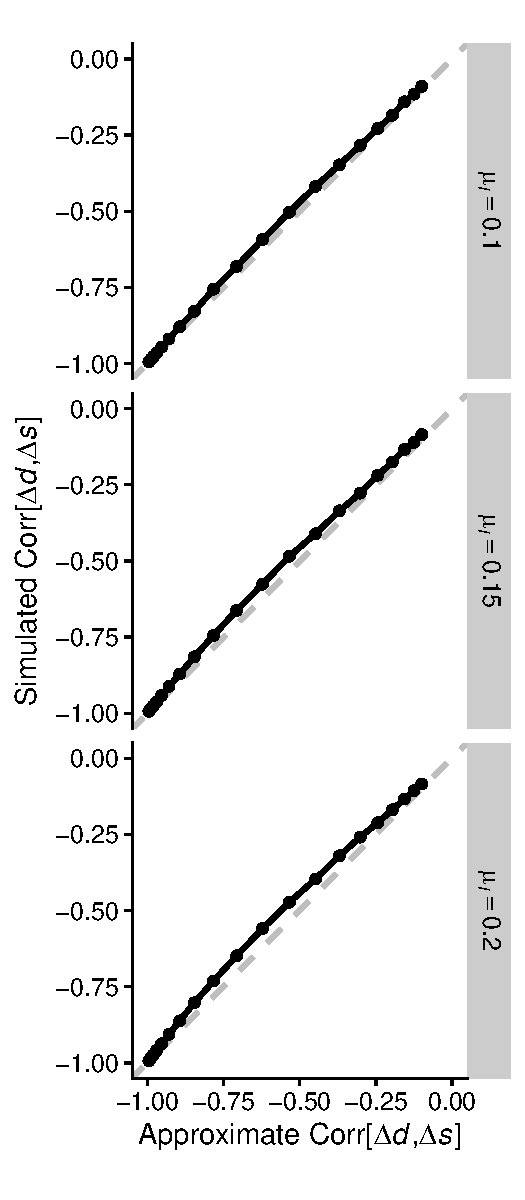
\includegraphics{../figures/check-approximation.pdf}
  \caption{(Caption next page.)}
  \label{fig:check-approximation}
\end{center}
\end{figure}
\addtocounter{figure}{-1}

\begin{figure} [t!]
\caption{(Previous page.) The approximation used to derive the correlation between log-transformed divergence in stomatal density and size ($\textrm{Corr}[\Delta d, \Delta s]$ in Eqn. \ref{eq:corr-ds1} matches simulated values. Each panel shows the relationship between approximate ($x$-axis) and calculated correlation values from $10^5$ random simulations per point ($y$-axis). The approximation is more accurate when the average stomatal index is low ($\mu_I = 0.1$) and less accurate when stomatal index is greater. Parameter values for simulations were $A = 5$, $B = 0.25$, $\mu_m = \textrm{log}[200~\mu\textrm{m}^3]$, $\sigma_{\Delta i} = 0.1$. The value of these parameters did not affect the results. The correlation changed based $\sigma_{\Delta m}$, which varied between 0.1 and 10 $\times~\sigma_{\Delta i}$).}
\end{figure}

\hypertarget{predictions}{%
\subsubsection{Predictions}\label{predictions}}

In this section, we summarize the predictions for each hypothesis (Table \ref{tab:predictions}) and show they can be difficult to distinguish under certain parameter combinations. Comparing the divergence of stomatal density and size on each surface provides additional evidence that can help resolve competing hypotheses. We can convert predictions from stomatal size to length using the relationship from Sack and Buckley (\protect\hyperlink{ref-sack_developmental_2016}{2016}): \(S = jL^2\) or \(s = \textrm{log}(j) + 2 l\) on the log-transformed scale. It follows that \(\Delta s = 2 \Delta l\), \(\textrm{Var}[\Delta s] = 4 \textrm{Var}[\Delta l]\), and \(\textrm{Corr}[\Delta d, \Delta s] = \textrm{Corr}[\Delta d, \Delta l]\).

\begin{table}[ht]
\caption{\label{tab:predictions}Key predictions about the (co)variance and correlation in divergence of log(stomatal density) ($\Delta d$) and log(stomatal size) ($\Delta s$) under the developmental integration and disintegration hypotheses. "Single surface" predictions apply to divergence in stomatal traits on either surface; "Both surfaces" predictions compare the divergence of traits on surface to that of the other. We further contrast two variants of the disintegration hypothesis, where either stomatal index ($\textrm{Var}[\Delta i] \ne 0$) or asymmetric cell division ($\textrm{Var}[\Delta b] \ne 0$) diverges.}
\begin{center}
\begin{tabular}{ccc}

\toprule
   & \multicolumn{2}{c}{Predictions} \\
  Hypothesis & Single surface & Both surfaces \\
  \midrule
  
  \multirow{3}{*}{Developmental integration} & \multicolumn{1}{c}{$\textrm{Var}[\Delta d] = \textrm{Var}[\Delta s]$} & \multicolumn{1}{c}{$\textrm{Var}[\Delta d_\textrm{ab}] = \textrm{Var}[\Delta d_\textrm{ad}]$} \\
& \multicolumn{1}{c}{$\textrm{Corr}[\Delta d, \Delta s] = -1$} & \multicolumn{1}{c}{$\textrm{Var}[\Delta s_\textrm{ad}] = \textrm{Var}[\Delta s_\textrm{ad}]$} \\  
& \multicolumn{1}{c}{} & \multicolumn{1}{c}{$\textrm{Cov}[\Delta d_\textrm{ab},\Delta s_\textrm{ab}] = \textrm{Cov}[\Delta d_\textrm{ad},\Delta s_\textrm{ad}]$} \\  

\midrule

  \multirow{2}{*}{Developmental disintegration} & \multicolumn{1}{c}{$\textrm{Var}[\Delta d] > \textrm{Var}[\Delta s]$} & \multicolumn{1}{c}{$\textrm{Var}[\Delta d_\textrm{ab}] \ne \textrm{Var}[\Delta d_\textrm{ad}]$} \\
& \multicolumn{1}{c}{$0 < \textrm{Corr}[\Delta d, \Delta s] < -1$} & \multicolumn{1}{c}{$\textrm{Var}[\Delta s_\textrm{ad}] = \textrm{Var}[\Delta s_\textrm{ad}]$} \\  
 $\textrm{Var}[\Delta i] \ne 0$ & \multicolumn{1}{c}{} & \multicolumn{1}{c}{$\textrm{Cov}[\Delta d_\textrm{ab},\Delta s_\textrm{ab}] \ne \textrm{Cov}[\Delta d_\textrm{ad},\Delta s_\textrm{ad}]$} \\  

\midrule

  \multirow{2}{*}{Developmental disintegration} & \multicolumn{1}{c}{$\textrm{Var}[\Delta d] < \textrm{Var}[\Delta s]$} & \multicolumn{1}{c}{$\textrm{Var}[\Delta d_\textrm{ab}] = \textrm{Var}[\Delta d_\textrm{ad}]$} \\
& \multicolumn{1}{c}{$0 < \textrm{Corr}[\Delta d, \Delta s] < -1$} & \multicolumn{1}{c}{$\textrm{Var}[\Delta s_\textrm{ad}] \ne \textrm{Var}[\Delta s_\textrm{ad}]$} \\  
 $\textrm{Var}[\Delta b] \ne 0$ & \multicolumn{1}{c}{} & \multicolumn{1}{c}{$\textrm{Cov}[\Delta d_\textrm{ab},\Delta s_\textrm{ab}] \ne \textrm{Cov}[\Delta d_\textrm{ad},\Delta s_\textrm{ad}]$} \\  

\bottomrule

\end{tabular}
\end{center}
\end{table}

The sections above clarify that it is possible to use the (co)divergence in stomatal density and size to test whether developmental integration contributes to phenotypic macroevolution. The problem is that there are parameter combinations where the (co)divergence in stomatal density and size appear consistent with strong developmental integration even when there is no constraint on the developmental function. For illustration, consider an extreme example where there is no divergence in \(m\) or \(a\) (\(\textrm{Var}[\Delta m] = \textrm{Var}[\Delta a] = 0\)) and the (co)variance in \(\Delta b\) and \(\Delta i\) are aligned such that \(\textrm{Var}[\Delta b] = \textrm{Var}[\Delta i] = -\textrm{Cov}[\Delta b, \Delta i]\)). This leads to the same predictions as the maximally constrained model, even though there is no constraint:

\begin{align}
  \textrm{Var}[\Delta s] = & \textrm{Var}[\Delta b] \\
  \textrm{Var}[\Delta d] = & \textrm{Var}[\Delta i] \\
  \textrm{Cov}[\Delta d, \Delta s] = & \textrm{Cov}[\Delta b, \Delta i] \\
  \textrm{Corr}[\Delta d, \Delta s] = & -1
\end{align}

Ideally, we would measure \(\Delta b\) and \(\Delta i\) to test whether they contribute significantly to divergence in stomatal density and size. This is challenging because comparative data on \(b\) and \(i\) is scarcer than that for \(d\) and \(s\). As a result, we can test whether \(\Delta b\) and \(\Delta i\) contribute in certain lineages but cannot directly quantify their relative importance for angiosperm macroevolution in general, as we attempt in this study.

We therefore take an alternative approach, leveraging the fact that stomatal trait evolution on each surface provides an additional line of evidence. If the stomatal developmental function is constrained then stomatal size and density on each surface should diverge in concert. Conversely, if the stomatal size and density on each surface diverge independently, this provides strong evidence that the developmental function is not fixed. If the developmental function differs between leaf surfaces with identical genomes then it seems implausible that it could not diverge over macroevolutionary time if there were selection. In that case we should give less credence to any hypothesis which posits that the developmental function \emph{cannot} evolve.

\clearpage

\hypertarget{notes-s2-phylogeny}{%
\subsection{Notes S2: Phylogeny}\label{notes-s2-phylogeny}}

We resolved taxonomic names using the R package \textbf{taxize} version 0.9.100 (\protect\hyperlink{ref-chamberlain_taxize_2013}{Chamberlain and Szöcs 2013}). We queried taxonomic names supplied by the original study authors on 2022-10-05 from the following sources: GRIN Taxonomy for Plants (\protect\hyperlink{ref-united_states_department_of_agriculture_agricultural_research_service_germplasm_2020}{United States Department of Agriculture, Agricultural Research Service 2020}), Open Tree of Life Reference Taxonomy (\protect\hyperlink{ref-rees_automated_2017}{Rees and Cranston 2017}), The International Plant Names Index (\protect\hyperlink{ref-the_royal_botanic_gardens_international_2020}{The Royal Botanic Gardens et al. 2020}), Tropicos - Missouri Botanical Garden (\protect\hyperlink{ref-missouri_botanical_garden_tropicos_2020}{Missouri Botanical Garden 2020}). We retained the maximum scoring matched name with taxize score \(\ge 0.75\) (a score of 1 is a perfect match). In 5 ambiguous cases we manually curated names. Taxonomic name resolution reduced the data set from 1120 to 1080 taxa. Most taxa are different species, but some recognized subspecies and varieties are also included. All algorithms and choices are documented in the associated source code.

We used the R packages \textbf{taxonlookup} version 1.1.5 (\protect\hyperlink{ref-pennell_simple_2016}{Pennell, FitzJohn, and Cornwell 2016}) and \textbf{V.phylomaker} version 0.1.0 (\protect\hyperlink{ref-jin_vphylomaker_2019}{Jin and Qian 2019}) to maximize overlap between our data set and the GBOTB.extended mega-tree of seed plants (\protect\hyperlink{ref-smith_constructing_2018}{Smith and Brown 2018}; \protect\hyperlink{ref-zanne_three_2014}{Zanne et al. 2014}). We further resolved large (\(\ge4\) taxa) polytomies in 29 clades with sufficient sequence data using \textbf{PyPHLAWD} version 1.0 (\protect\hyperlink{ref-smith_pyphlawd_2019}{Smith and Walker 2019}) in Python 3.9.2 (Python Software Foundation, \url{https://www.python.org/}). We used sequence data from the most recent GenBank Plant and Fungal sequences database division (\protect\hyperlink{ref-ouellette_database_1997}{Ouellette and Boguski 1997}). We inferred subtree phylogenies using RAxML version 8.2.12 (\protect\hyperlink{ref-stamatakis_raxml_2014}{Stamatakis 2014}) and conducted molecular dating using the \texttt{chronos()} function in the R package \textbf{ape} version 5.6.2 (\protect\hyperlink{ref-paradis_ape_2019}{Paradis and Schliep 2019}) to obtain ultrametric trees. We grafted resolved, ultrametric subtrees onto the mega-tree at the polytomy nodes and rescaled to keep the mega-tree ultrametric. In some cases, resolving polytomies was not possible because there was little or no overlap between taxa in the data set and taxa with sequence data available for \textbf{PyPHLAWD}. In these cases, we randomly selected two taxa as a phylogenetially independent pair and dropped the rest. Remaining polytomies of three taxa were resolved randomly using the \texttt{multi2di()} function in \textbf{ape}. The final data set for which we had both trait and phylogenetic information contained 638 taxa (Notes S3).

\clearpage

\begin{longtable}[]{@{}ll@{}}
\caption{\label{tab:sources}Primary sources of stomatal anatomical data and the taxa covered by each source.}\tabularnewline
\toprule()
Source & Taxa \\
\midrule()
\endfirsthead
\toprule()
Source & Taxa \\
\midrule()
\endhead
Arambarri et al. (\protect\hyperlink{ref-arambarri_taxonomy_2005}{2005}) & lotus \\
Avita and Inamdar (\protect\hyperlink{ref-avita_structure_1980}{1980}) & ranunculaceae,paeoniaceae \\
Bucher et al. (\protect\hyperlink{ref-bucher_stomatal_2017}{2017}) & many \\
Caldera et al. (\protect\hyperlink{ref-caldera_effects_2017}{2017}) & arabidopsis thaliana \\
Chandra (\protect\hyperlink{ref-chandra_epidermal_1967}{1967}) & solanum \\
Conesa et al. (\protect\hyperlink{ref-conesa_stomatal_2019}{2019}) & limonium \\
Eckerson (\protect\hyperlink{ref-eckerson_number_1908}{1908}) & many \\
Gindel (\protect\hyperlink{ref-gindel_stomatal_1969}{1969}) & many \\
Giuliani et al. (\protect\hyperlink{ref-giuliani_coordination_2013}{2013}) & oryza \\
Hanafy et al. (\protect\hyperlink{ref-hanafy_leaf_2019}{2019}) & mentha \\
Huang (\protect\hyperlink{ref-huang_leaf_2019}{2019}) & trees \\
Juhász (\protect\hyperlink{ref-juhasz_effect_1966}{1966}) & solanum \\
Juhász (\protect\hyperlink{ref-juhasz_comparative_1968}{1968}) & solanum \\
Kannabiran and Ramassamy (\protect\hyperlink{ref-kannabiran_foliar_1988}{1988}) & apocynaceae \\
Kawamitsu et al. (\protect\hyperlink{ref-kawamitsu_stomatal_1996}{1996}) & grasses \\
Khan et al. (\protect\hyperlink{ref-khan_taxonomic_2019}{2019}) & gymnosperms \\
Kim (\protect\hyperlink{ref-kim_comparative_1987}{1987}) & silverswords \\
McKown, Akamine, and Sack (\protect\hyperlink{ref-mckown_trait_2016}{2016}) & scaevola \\
Muir, Galmés, and Conesa (\protect\hyperlink{ref-muir_unpublished_2022}{2022}) & solanum \\
Pallardy and Kozlowski (\protect\hyperlink{ref-pallardy_frequency_1979}{1979}) & populus \\
Pandey and Nagar (\protect\hyperlink{ref-pandey_patterns_2003}{2003}) & many \\
Pathare, Koteyeva, and Cousins (\protect\hyperlink{ref-pathare_increased_2020}{2020}) & grasses \\
Rivera, Villaseñor, and Terrazas (\protect\hyperlink{ref-rivera_meso-_2017}{2017}) & asteraceae \\
Rodriguez (\protect\hyperlink{ref-rodriguez_unpublished_2021}{2021}) & eucalyptus \\
Scalon et al. (\protect\hyperlink{ref-scalon_leaf_2016}{2016}) & passovia \\
Siddiqi, Ahmad, and Rehman (\protect\hyperlink{ref-siddiqi_contribution_1991}{1991}) & euphorbiaceae \\
Sporck (\protect\hyperlink{ref-sporck_hawaiian_2011}{2011}) & euphorbia \\
Stenglein et al. (\protect\hyperlink{ref-stenglein_leaf_2003}{2003a}) & lotus \\
Stenglein et al. (\protect\hyperlink{ref-stenglein_leaf_2003-1}{2003b}) & lotus \\
Sundberg (\protect\hyperlink{ref-sundberg_comparison_1986}{1986}) & many \\
Szymura and Wolski (\protect\hyperlink{ref-szymura_leaf_2011}{2011}) & solidago \\
Xiong and Flexas (\protect\hyperlink{ref-xiong_one_2020}{2020}) & many \\
Yang et al. (\protect\hyperlink{ref-yang_large-scale_2014}{2014}) & many \\
Zarinkamar (\protect\hyperlink{ref-zarinkamar_density_2006}{2006}) & monocots \\
Zarinkamar (\protect\hyperlink{ref-zarinkamar_stomatal_2007}{2007}) & eudicots \\
Zhao et al. (\protect\hyperlink{ref-zhao_difference_2020}{2020}) & monocots \\
Zlatković et al. (\protect\hyperlink{ref-zlatkovic_epidermal_2017}{2017}) & sedum \\
Zoric et al. (\protect\hyperlink{ref-zoric_leaf_2009}{2009}) & trifolium \\
\bottomrule()
\end{longtable}

\clearpage

\hypertarget{references-cited-only-in-the-online-enhancements}{%
\section*{References Cited Only in the Online Enhancements}\label{references-cited-only-in-the-online-enhancements}}
\addcontentsline{toc}{section}{References Cited Only in the Online Enhancements}

\hypertarget{refs}{}
\begin{CSLReferences}{1}{0}
\leavevmode\vadjust pre{\hypertarget{ref-arambarri_taxonomy_2005}{}}%
Arambarri, Ana M., Sebastián A. Stenglein, Marta N. Colares, and María C. Novoa. 2005. {``Taxonomy of the {New} {World} Species of {Lotus} ({Leguminosae}: {Loteae}).''} \emph{Australian Journal of Botany} 53 (8): 797. \url{https://doi.org/10.1071/BT04101}.

\leavevmode\vadjust pre{\hypertarget{ref-avita_structure_1980}{}}%
Avita, S. R., and J. A. Inamdar. 1980. {``Structure and {Ontogeny} of {Stomata} in {Ranunculaceae} and {Paeoniaceae}.''} \emph{Flora} 170 (4): 354--70. \url{https://doi.org/10.1016/S0367-2530(17)31224-0}.

\leavevmode\vadjust pre{\hypertarget{ref-bergmann_stomatal_2007}{}}%
Bergmann, Dominique C., and Fred D. Sack. 2007. {``Stomatal {Development}.''} \emph{Annual Review of Plant Biology} 58 (1): 163--81. \url{https://doi.org/10.1146/annurev.arplant.58.032806.104023}.

\leavevmode\vadjust pre{\hypertarget{ref-bucher_stomatal_2017}{}}%
Bucher, Solveig Franziska, Karl Auerswald, Christina Grün-Wenzel, Steven I. Higgins, Javier Garcia Jorge, and Christine Römermann. 2017. {``Stomatal Traits Relate to Habitat Preferences of Herbaceous Species in a Temperate Climate.''} \emph{Flora} 229 (April): 107--15. \url{https://doi.org/10.1016/j.flora.2017.02.011}.

\leavevmode\vadjust pre{\hypertarget{ref-caldera_effects_2017}{}}%
Caldera, H. Iroja U., W. A. Janendra M. De Costa, F. Ian Woodward, Janice A. Lake, and Sudheera M. W. Ranwala. 2017. {``Effects of Elevated Carbon Dioxide on Stomatal Characteristics and Carbon Isotope Ratio of \emph{{Arabidopsis} Thaliana} Ecotypes Originating from an Altitudinal Gradient.''} \emph{Physiologia Plantarum} 159 (1): 74--92. \url{https://doi.org/10.1111/ppl.12486}.

\leavevmode\vadjust pre{\hypertarget{ref-chamberlain_taxize_2013}{}}%
Chamberlain, Scott A., and Eduard Szöcs. 2013. {``Taxize: Taxonomic Search and Retrieval in {R}.''} \emph{F1000Research} 2 (October): 191. \url{https://doi.org/10.12688/f1000research.2-191.v2}.

\leavevmode\vadjust pre{\hypertarget{ref-chandra_epidermal_1967}{}}%
Chandra, V. 1967. {``Epidermal Studies on Some {Solanaceous} Plants.''} \emph{Indian Journal of Pharmacy} 29: 227--29.

\leavevmode\vadjust pre{\hypertarget{ref-conesa_stomatal_2019}{}}%
Conesa, Miquel À, Christopher D Muir, Arantzazu Molins, and Jeroni Galmés. 2019. {``Stomatal Anatomy Coordinates Leaf Size with {Rubisco} Kinetics in the {Balearic} {Limonium}.''} \emph{AoB PLANTS}, August, plz050. \url{https://doi.org/10.1093/aobpla/plz050}.

\leavevmode\vadjust pre{\hypertarget{ref-dow_patterning_2014}{}}%
Dow, Graham J., and Dominique C. Bergmann. 2014. {``Patterning and Processes: How Stomatal Development Defines Physiological Potential.''} \emph{Current Opinion in Plant Biology} 21 (October): 67--74. \url{https://doi.org/10.1016/j.pbi.2014.06.007}.

\leavevmode\vadjust pre{\hypertarget{ref-dow_integrated_2014}{}}%
Dow, Graham J., Dominique C. Bergmann, and Joseph A. Berry. 2014. {``An Integrated Model of Stomatal Development and Leaf Physiology.''} \emph{New Phytologist} 201 (4): 1218--26.

\leavevmode\vadjust pre{\hypertarget{ref-eckerson_number_1908}{}}%
Eckerson, Sophia H. 1908. {``The Number and Size of the Stomata.''} \emph{Botanical Gazette} 46 (3): 221--24.

\leavevmode\vadjust pre{\hypertarget{ref-gindel_stomatal_1969}{}}%
Gindel, I. 1969. {``Stomatal Number and Size as Related to Soil Moisture in Tree Xerophytes in {Israel}.''} \emph{Ecology} 50 (2): 263--67.

\leavevmode\vadjust pre{\hypertarget{ref-giuliani_coordination_2013}{}}%
Giuliani, Rita, Nuria Koteyeva, Elena Voznesenskaya, Marc A Evans, Asaph B Cousins, and Gerald E Edwards. 2013. {``Coordination of Leaf Photosynthesis, Transpiration, and Structural Traits in Rice and Wild Relatives (Genus \emph{o}ryza).''} \emph{Plant Physiology} 162 (3): 1632--51.

\leavevmode\vadjust pre{\hypertarget{ref-hanafy_leaf_2019}{}}%
Hanafy, Doaa M., Paul D. Prenzler, Rodney A. Hill, and Geoffrey E. Burrows. 2019. {``Leaf Micromorphology of 19 {Mentha} Taxa.''} \emph{Australian Journal of Botany} 67 (7): 463. \url{https://doi.org/10.1071/BT19054}.

\leavevmode\vadjust pre{\hypertarget{ref-huang_leaf_2019}{}}%
Huang, Sophia. 2019. {``Leaf Functional Traits as Predictors of Drought Tolerance in Urban Trees.''} Master's thesis, San Luis Obispo: California Polytechnic State University, San Luis Obispo.

\leavevmode\vadjust pre{\hypertarget{ref-jin_vphylomaker_2019}{}}%
Jin, Yi, and Hong Qian. 2019. {``V.{PhyloMaker}: An {R} Package That Can Generate Very Large Phylogenies for Vascular Plants.''} \emph{Ecography} 42 (8): 1353--59. \url{https://doi.org/10.1111/ecog.04434}.

\leavevmode\vadjust pre{\hypertarget{ref-juhasz_effect_1966}{}}%
Juhász, M. 1966. {``Effect of Ecological Factors on the Leaf Epidermis of Species {Solanum}.''} \emph{Acta Biologica} 12 (3-4): 29--36.

\leavevmode\vadjust pre{\hypertarget{ref-juhasz_comparative_1968}{}}%
---------. 1968. {``A Comparative Histological Examination of the Leaf Epidermis of Some {Solanum} Species.''} \emph{Acta Biologica} 14: 5--9.

\leavevmode\vadjust pre{\hypertarget{ref-kannabiran_foliar_1988}{}}%
Kannabiran, B, and V Ramassamy. 1988. {``Foliar Epidermis and Taxonomy in {Apocynaceae}.''} \emph{Proceedings of the Indian Academy of Sciences} 98 (5): 409--17.

\leavevmode\vadjust pre{\hypertarget{ref-kawamitsu_stomatal_1996}{}}%
Kawamitsu, Yoshinobu, Shin-ichi Hiyane, Seiichi Murayama, Akihiro Nose, and Choyu Shinjyo. 1996. {``Stomatal Frequency and Guard Cell Length in {C}\(_{\textrm{3}}\) and {C}\(_{\textrm{4}}\) Grass Species.''} \emph{Japanese Journal of Crop Science} 65 (4): 626--33.

\leavevmode\vadjust pre{\hypertarget{ref-khan_taxonomic_2019}{}}%
Khan, Raees, Sheikh Zain Ul Abidin, Mushtaq Ahmad, Muhammad Zafar, Jie Liu, Lubna, Shayan Jamshed, and Ömer Kiliç. 2019. {``Taxonomic Importance of {SEM} and {LM} Foliar Epidermal Micro-Morphology: {A} Tool for Robust Identification of Gymnosperms.''} \emph{Flora} 255 (June): 42--68. \url{https://doi.org/10.1016/j.flora.2019.03.016}.

\leavevmode\vadjust pre{\hypertarget{ref-kim_comparative_1987}{}}%
Kim, Insun. 1987. {``Comparative {Anatomy} of {Some} {Parents} and {Hybrids} of the {Hawaiian} {Madiinae} ({Asteraceae}).''} \emph{American Journal of Botany} 74 (8): 1224--38. \url{https://doi.org/10.2307/2444158}.

\leavevmode\vadjust pre{\hypertarget{ref-lynch_genetics_1998}{}}%
Lynch, Michael, and Bruce Walsh. 1998. \emph{Genetics and Analysis of Quantitative Traits}. Sunderland, Mass: Sinauer.

\leavevmode\vadjust pre{\hypertarget{ref-mckown_trait_2016}{}}%
McKown, Athena D., Michelle Elmore Akamine, and Lawren Sack. 2016. {``Trait Convergence and Diversification Arising from a Complex Evolutionary History in {Hawaiian} Species of {Scaevola}.''} \emph{Oecologia} 181 (4): 1083--1100. \url{https://doi.org/10.1007/s00442-016-3640-3}.

\leavevmode\vadjust pre{\hypertarget{ref-missouri_botanical_garden_tropicos_2020}{}}%
Missouri Botanical Garden. 2020. {``Tropicos.''} \url{https://tropicos.org}.

\leavevmode\vadjust pre{\hypertarget{ref-muir_unpublished_2022}{}}%
Muir, Christopher D, Jeroni Galmés, and Miquel À Conesa. 2022. {``Unpublished Data.''}

\leavevmode\vadjust pre{\hypertarget{ref-ouellette_database_1997}{}}%
Ouellette, B. F. Francis, and Mark S. Boguski. 1997. {``Database {Divisions} and {Homology} {Search} {Files}: {A} {Guide} for the {Perplexed}.''} \emph{Genome Research} 7 (10): 952--55. \url{https://doi.org/10.1101/gr.7.10.952}.

\leavevmode\vadjust pre{\hypertarget{ref-pallardy_frequency_1979}{}}%
Pallardy, S G, and T T Kozlowski. 1979. {``Frequency and Length of Stomata of 21 {Populus} Clones.''} \emph{Canadian Journal of Botany} 57: 2519--23.

\leavevmode\vadjust pre{\hypertarget{ref-pandey_patterns_2003}{}}%
Pandey, Subedar, and Pramod Kumar Nagar. 2003. {``Patterns of Leaf Surface Wetness in Some Important Medicinal and Aromatic Plants of {Western} {Himalaya}.''} \emph{Flora} 198: 349--57.

\leavevmode\vadjust pre{\hypertarget{ref-paradis_ape_2019}{}}%
Paradis, Emmanuel, and Klaus Schliep. 2019. {``Ape 5.0: An Environment for Modern Phylogenetics and Evolutionary Analyses in {R}.''} Edited by Russell Schwartz. \emph{Bioinformatics} 35 (3): 526--28. \url{https://doi.org/10.1093/bioinformatics/bty633}.

\leavevmode\vadjust pre{\hypertarget{ref-pathare_increased_2020}{}}%
Pathare, Varsha S., Nuria Koteyeva, and Asaph B. Cousins. 2020. {``Increased Adaxial Stomatal Density Is Associated with Greater Mesophyll Surface Area Exposed to Intercellular Air Spaces and Mesophyll Conductance in Diverse {C} \(_{\textrm{4}}\) Grasses.''} \emph{New Phytologist} 225 (1): 169--82. \url{https://doi.org/10.1111/nph.16106}.

\leavevmode\vadjust pre{\hypertarget{ref-pennell_simple_2016}{}}%
Pennell, Matthew W, Richard G FitzJohn, and William K Cornwell. 2016. {``A Simple Approach for Maximizing the Overlap of Phylogenetic and Comparative Data.''} \emph{Methods in Ecology and Evolution} 7 (6): 751--58.

\leavevmode\vadjust pre{\hypertarget{ref-price_correlations_1973}{}}%
Price, H. J., A. H. Sparrow, and Anne F. Nauman. 1973. {``Correlations Between Nuclear Volume, Cell Volume and {DNA} Content in Meristematic Cells of Herbaceous Angiosperms.''} \emph{Experientia} 29 (8): 1028--29. \url{https://doi.org/10.1007/BF01930444}.

\leavevmode\vadjust pre{\hypertarget{ref-rees_automated_2017}{}}%
Rees, Jonathan, and Karen Cranston. 2017. {``Automated Assembly of a Reference Taxonomy for Phylogenetic Data Synthesis.''} \emph{Biodiversity Data Journal} 5 (May): e12581. \url{https://doi.org/10.3897/BDJ.5.e12581}.

\leavevmode\vadjust pre{\hypertarget{ref-rivera_meso-_2017}{}}%
Rivera, Patricia, José Luis Villaseñor, and Teresa Terrazas. 2017. {``Meso- or Xeromorphic? {Foliar} Characters of {Asteraceae} in a Xeric Scrub of {Mexico}.''} \emph{Botanical Studies} 58 (1): 12. \url{https://doi.org/10.1186/s40529-017-0166-x}.

\leavevmode\vadjust pre{\hypertarget{ref-rodriguez_unpublished_2021}{}}%
Rodriguez, Rosana Ana Lopez. 2021. {``Unpublished Data.''}

\leavevmode\vadjust pre{\hypertarget{ref-sack_developmental_2016}{}}%
Sack, Lawren, and Thomas N Buckley. 2016. {``The Developmental Basis of Stomatal Density and Flux.''} \emph{Plant Physiology} 171 (4): 2358--63. \url{https://doi.org/10.1104/pp.16.00476}.

\leavevmode\vadjust pre{\hypertarget{ref-scalon_leaf_2016}{}}%
Scalon, Marina Corrêa, Davi Rodrigo Rossatto, Fabricius Maia Chaves Bicalho Domingos, and Augusto Cesar Franco. 2016. {``Leaf Morphophysiology of a {Neotropical} Mistletoe Is Shaped by Seasonal Patterns of Host Leaf Phenology.''} \emph{Oecologia} 180 (4): 1103--12. \url{https://doi.org/10.1007/s00442-015-3519-8}.

\leavevmode\vadjust pre{\hypertarget{ref-siddiqi_contribution_1991}{}}%
Siddiqi, M Rehan, Shabbir Ahmad, and Zia-Ul Rehman. 1991. {``A Contribution to the Study of Epidermis in Some Members of the Family {Euphorbiaceae}.''} In \emph{Plant {Life} of {South} {Asia}}, 169--82.

\leavevmode\vadjust pre{\hypertarget{ref-simova_geometrical_2012}{}}%
Šímová, Irena, and Tomáš Herben. 2012. {``Geometrical Constraints in the Scaling Relationships Between Genome Size, Cell Size and Cell Cycle Length in Herbaceous Plants.''} \emph{Proceedings of the Royal Society B: Biological Sciences} 279 (1730): 867--75. \url{https://doi.org/10.1098/rspb.2011.1284}.

\leavevmode\vadjust pre{\hypertarget{ref-smith_constructing_2018}{}}%
Smith, Stephen A., and Joseph W. Brown. 2018. {``Constructing a Broadly Inclusive Seed Plant Phylogeny.''} \emph{American Journal of Botany} 105 (3): 302--14. \url{https://doi.org/10.1002/ajb2.1019}.

\leavevmode\vadjust pre{\hypertarget{ref-smith_pyphlawd_2019}{}}%
Smith, Stephen A., and Joseph F. Walker. 2019. {``{PyPHLAWD}: {A} Python Tool for Phylogenetic Dataset Construction.''} Edited by Natalie Cooper. \emph{Methods in Ecology and Evolution} 10 (1): 104--8. \url{https://doi.org/10.1111/2041-210X.13096}.

\leavevmode\vadjust pre{\hypertarget{ref-sporck_hawaiian_2011}{}}%
Sporck, Margaret J. 2011. {``The {Hawaiian} {C}\(_{\textrm{4}}\) \emph{Euphorbia} Adaptive Radiation: An Ecophysiological Approach to Understanding Leaf Trait Variation.''} Ph.\{D\}., University of Hawaii.

\leavevmode\vadjust pre{\hypertarget{ref-stamatakis_raxml_2014}{}}%
Stamatakis, Alexandros. 2014. {``{RAxML} Version 8: A Tool for Phylogenetic Analysis and Post-Analysis of Large Phylogenies.''} \emph{Bioinformatics} 30 (9): 1312--13.

\leavevmode\vadjust pre{\hypertarget{ref-stenglein_leaf_2003}{}}%
Stenglein, Sebastián A, Ana M Arambarri, Marta N Colares, María C Novoa, and Claudia E Vizcaíno. 2003a. {``Leaf Epidermal Characteristics of \emph{Lotus} Subgenus \emph{Acmispon} ({Fabaceae}: {Loteae}) and a Numerical Taxonomic Evaluation.''} \emph{Canadian Journal of Botany} 81 (9): 933--44. \url{https://doi.org/10.1139/b03-090}.

\leavevmode\vadjust pre{\hypertarget{ref-stenglein_leaf_2003-1}{}}%
---------. 2003b. {``Leaf Epidermal Characteristics of \emph{Lotus} Subgenus \emph{Acmispon} ({Fabaceae}: {Loteae}) and a Numerical Taxonomic Evaluation.''} \emph{Canadian Journal of Botany} 81 (9): 933--44. \url{https://doi.org/10.1139/b03-090}.

\leavevmode\vadjust pre{\hypertarget{ref-sundberg_comparison_1986}{}}%
Sundberg, Marshall D. 1986. {``A Comparison of Stomatal Distribution and Length in Succulent and Non-Succulent Desert Plants.''} \emph{Phytomorphology} 36 (1-2): 53--66.

\leavevmode\vadjust pre{\hypertarget{ref-szymura_leaf_2011}{}}%
Szymura, Magdalena, and Karol Wolski. 2011. {``Leaf {Epidermis} {Traits} as {Tools} to {Identify} {Solidago} {L}. {Taxa} in {Poland}.''} \emph{Acta Biologica Cracoviensia Series Botanica} 53 (1). \url{https://doi.org/10.2478/v10182-011-0006-3}.

\leavevmode\vadjust pre{\hypertarget{ref-the_royal_botanic_gardens_international_2020}{}}%
The Royal Botanic Gardens, Kew, Harvard University Herbaria \& Libraries, and Australian National Botanic Gardens. 2020. {``International {Plant} {Names} {Index}.''} \url{http://www.ipni.org}.

\leavevmode\vadjust pre{\hypertarget{ref-united_states_department_of_agriculture_agricultural_research_service_germplasm_2020}{}}%
United States Department of Agriculture, Agricultural Research Service. 2020. {``Germplasm {Resources} {Information} {Network}.''} \url{http://www.ars-grin.gov/.}

\leavevmode\vadjust pre{\hypertarget{ref-wagner_multivariate_1989}{}}%
Wagner, G P. 1989. {``Multivariate Mutation-Selection Balance with Constrained Pleiotropic Effects.''} \emph{Genetics} 122 (1): 223--34. \url{https://doi.org/10.1093/genetics/122.1.223}.

\leavevmode\vadjust pre{\hypertarget{ref-xiong_one_2020}{}}%
Xiong, Dongliang, and Jaume Flexas. 2020. {``From One Side to Two Sides: The Effects of Stomatal Distribution on Photosynthesis.''} \emph{New Phytologist} 228 (6): 1754--66. \url{https://doi.org/10.1111/nph.16801}.

\leavevmode\vadjust pre{\hypertarget{ref-yang_large-scale_2014}{}}%
Yang, Xiaoxia, Ya Yang, Chengjun Ji, Tao Feng, Yue Shi, Li Lin, Jianjing Ma, and Jin-Sheng He. 2014. {``Large-Scale Patterns of Stomatal Traits in {Tibetan} and {Mongolian} Grassland Species.''} \emph{Basic and Applied Ecology} 15 (2): 122--32. \url{https://doi.org/10.1016/j.baae.2014.01.003}.

\leavevmode\vadjust pre{\hypertarget{ref-zanne_three_2014}{}}%
Zanne, Amy E., David C. Tank, William K. Cornwell, Jonathan M. Eastman, Stephen A. Smith, Richard G. FitzJohn, Daniel J. McGlinn, et al. 2014. {``Three Keys to the Radiation of Angiosperms into Freezing Environments.''} \emph{Nature} 506 (7486): 89--92. \url{https://doi.org/10.1038/nature12872}.

\leavevmode\vadjust pre{\hypertarget{ref-zarinkamar_density_2006}{}}%
Zarinkamar, Fatemeh. 2006. {``Density, Size and Distribution of Stomata in Different Monocotyledons.''} \emph{Pakistan Journal of Biological Sciences} 9 (9): 1650--59.

\leavevmode\vadjust pre{\hypertarget{ref-zarinkamar_stomatal_2007}{}}%
---------. 2007. {``Stomatal Observations in Dicotyledons.''} \emph{Pakistan Journal of Biological Sciences} 10 (2): 199--219.

\leavevmode\vadjust pre{\hypertarget{ref-zhao_difference_2020}{}}%
Zhao, Wanli, Peili Fu, Guolan Liu, and Ping Zhao. 2020. {``Difference Between Emergent Aquatic and Terrestrial Monocotyledonous Herbs in Relation to the Coordination of Leaf Stomata with Vein Traits.''} Edited by Kristine Crous. \emph{AoB PLANTS} 12 (5): plaa047. \url{https://doi.org/10.1093/aobpla/plaa047}.

\leavevmode\vadjust pre{\hypertarget{ref-zlatkovic_epidermal_2017}{}}%
Zlatković, B., Z. S. Mitić, S. Jovanović, D. Lakušić, B. Lakušić, J. Rajković, and G. Stojanović. 2017. {``Epidermal Structures and Composition of Epicuticular Waxes of \emph{{Sedum} Album Sensu Lato} ({Crassulaceae}) in {Balkan} {Peninsula}.''} \emph{Plant Biosystems - An International Journal Dealing with All Aspects of Plant Biology} 151 (6): 974--84. \url{https://doi.org/10.1080/11263504.2016.1218971}.

\leavevmode\vadjust pre{\hypertarget{ref-zoric_leaf_2009}{}}%
Zoric, Lana, Ljiljana Merkulov, Jadranka Lukovic, Pal Boza, and Dubravka Polic. 2009. {``Leaf Epidermal Characteristics of {Trifolium} {L}. Species from {Serbia} and {Montenegro}.''} \emph{Flora - Morphology, Distribution, Functional Ecology of Plants} 204 (3): 198--209. \url{https://doi.org/10.1016/j.flora.2008.02.002}.

\end{CSLReferences}

\end{document}
